\subsection{Server Subsystem}
The system records the users voice sound and send it to sever. 
Sever compare the sound with the database and calculate the difference and send back to the application.

\begin{figure}[h!]
	\centering
 	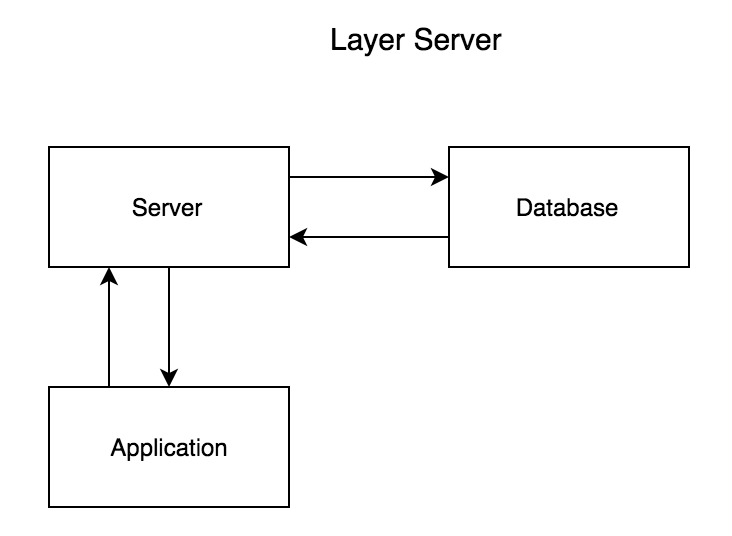
\includegraphics[width=0.60\textwidth]{images/subsystem_server}
 \caption{Server subsystem diagram}
\end{figure}

\subsubsection{Assumptions}
The Server receive the user's voice data and compare data with the standard voice data from the database.

\subsubsection{Responsibilities}
The application sends the voice data to the server.
The sever get data from the database and calculate the difference, then send the information back.
The application records the user's sound, and send to the server, and when sever received the user's voice data, then compare data with the standard voice data from the database. The server send back the \% difference to the application.

\subsubsection{Subsystem Interfaces}
\begin {table}[H]
\caption {Server Subsystem interfaces} 
\begin{center}
    \begin{tabular}{ | p{1cm} | p{6cm} | p{3cm} | p{3cm} |}
    \hline
    ID & Description & Inputs & Outputs \\ \hline
    \#1 & Display the graph dot by calculate the difference of the voice words & \pbox{3cm}{Voice Words} & \pbox{3cm}{Graph Dot}  \\ \hline
    \end{tabular}
\end{center}
\end{table}
